\section{Mikrofone}
\label{sec:1}
In dieser Hausaufgabe werden die akustischen Eigenschaften einer Auswahl an Mikrofonen (siehe Tabelle \ref{tab:mics}) analysiert und miteinander verglichen.
Als Grundlage stehen die Frequenzgangsdaten für den Schalldruckpegel aus verschieden Einfallsrichtungen zur Verfügung.

\def\arraystretch{1.5}
\begin{table}[h]
    \centering
    \caption{Auswahl der Mikrofone}
    \label{tab:mics}
    \begin{tabular}{l l l l l}
        Hersteller & Typ & Akustische Arbeitsweise & Richtcharakteristik & Einfallsrichtungen \\
        \hline
        Shure & \texttt{SM58} & Druckgradienten- und Schnelleempfänger & Niere & 0°, 90°, 180° \\
        Neumann & \texttt{KM120} & Druckgradienten- und Auslenkungsempfänger & Acht & 0°, 90°, 180° \\
        Neumann & \texttt{KM184} & Druckgradienten- und Auslenkungsempfänger & Niere & 0°, 5°, ..., 180°
    \end{tabular}
\end{table}


\subsection{\texttt{K120} und \texttt{SM58} bei Frontalschalleinfall}

Die Abbildung \ref{fig:freq_0} zeigt die auf 1000 Hz normierten Frequenzgänge der Mikrophone bei Frontalschalleinfall.


\begin{figure}[b]
    \centering
    \begin{subfigure}{.5\textwidth}
        \centering
        \caption{KM120}
        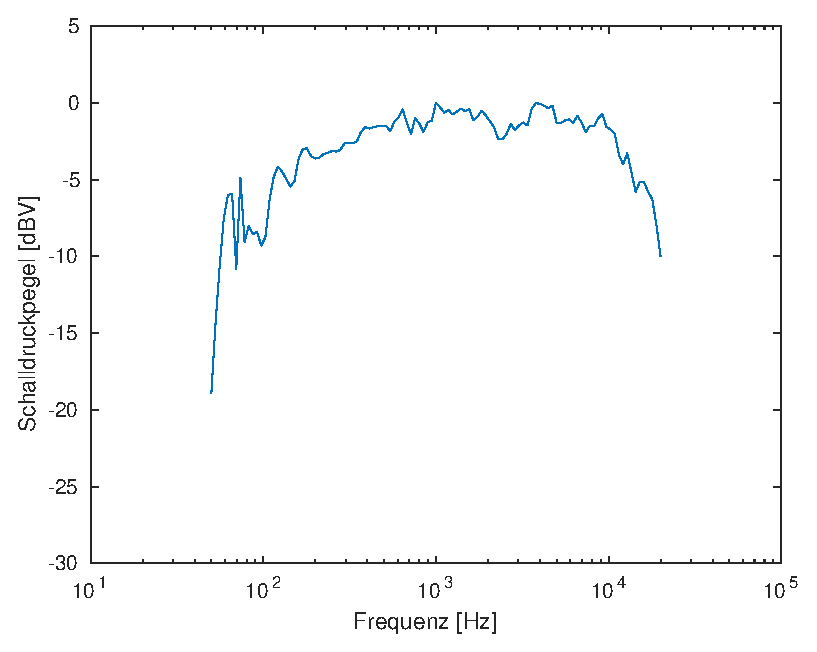
\includegraphics[width=0.95\linewidth]{Figures/km120_0}
    \end{subfigure}%
    \begin{subfigure}{.5\textwidth}
        \centering
        \caption{SM58}
        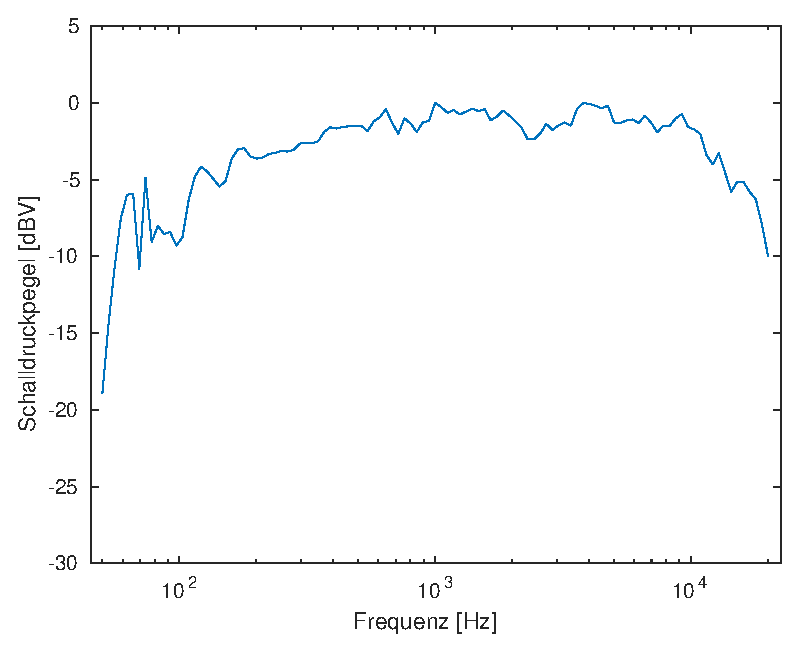
\includegraphics[width=0.95\linewidth]{Figures/sm58_0}
    \end{subfigure}
    \caption{Frequenzgänge der Mikrofone bei Frontalschalleinfall normiert auf 0 dBV bei 1000 Hz}
    \label{fig:freq_0}
\end{figure}

\subsection{Glättung der Frequenzgänge}
Für die Implementierung des gleitenden Mittelwerts verwenden wir Matlabs \texttt{MovMean()} Methode.
Das resultierende, geglättete Spektrum ist in Abbildung \ref{fig:freq_movmean} zu sehen. Das Verhältnis benachbarter Frequenzbins ist konstant und beträgt $f_{n+1}/f_{n} = 1.057$.
Die Frequenzauflösung der Spektren ist somit nicht linear, sondern abhängig von der Frequenz.
Zudem mittelt der gleitende Mittelwert konstant über drei Bins.
Das bedeutet, dass es sich um eine Glättung mit relativer Bandbreite handelt.
Allerdings ist es weder eine terzbreite noch eine oktavbreite Glättung.
In beiden Fällen müsste das Frequenzverhältnis benachbarter Bins größer sein.
Allgemein gilt: Eine Glättung mit relativer Bandbreite liefert eine gleichmäßigere Kurve in logarithmischer Darstellung der Frequenzachse des Spektrums, als eine Glättung mit konstanter Bandbreite.
Letztere liefert wiederum eine gleichmäßig geglättete Kurve für eine Darstellung mit linearer Frequenzachse.

\begin{figure}[b]
    \centering
    \begin{subfigure}{.5\textwidth}
        \centering
        \caption{KM120}
        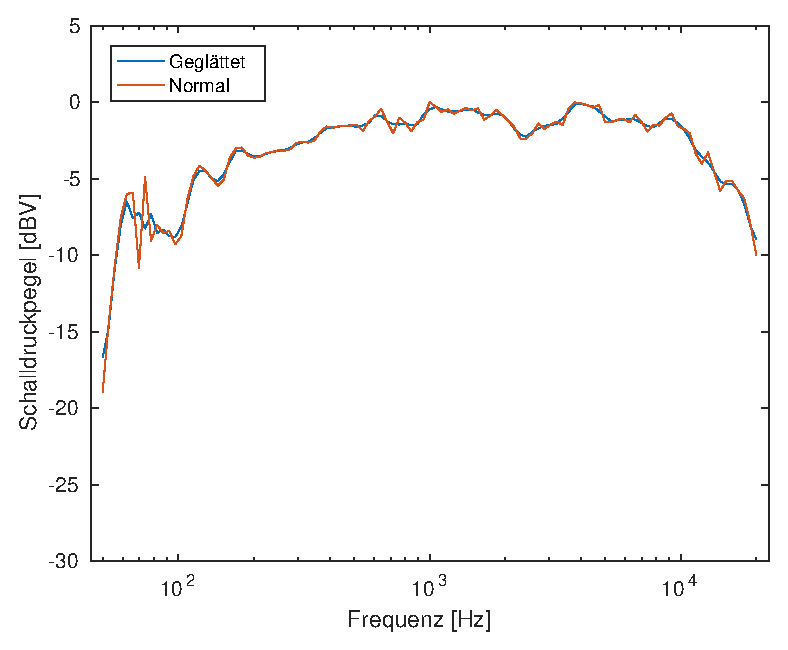
\includegraphics[width=0.95\linewidth]{Figures/km120_0_movmean}
    \end{subfigure}%
    \begin{subfigure}{.5\textwidth}
        \centering
        \caption{SM58}
        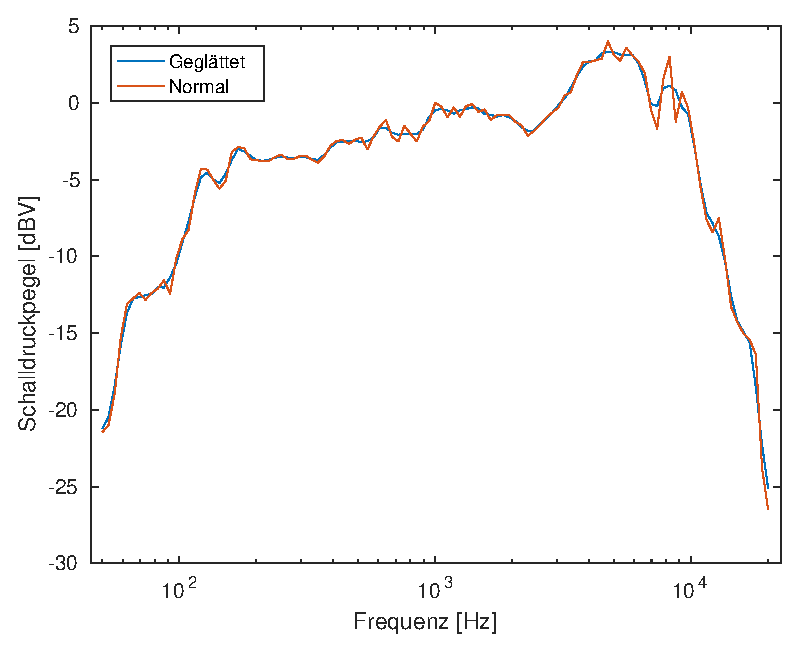
\includegraphics[width=0.95\linewidth]{Figures/sm58_0_movmean}
    \end{subfigure}
    \caption{Unterschied zwischen dem normalen und dem geglätteten Frequenzgang der Mikrofone bei frontalem Schalleinfall}
    \label{fig:freq_movmean}
\end{figure}

\subsection{Weitere Einfallsrichtungen}

Die Abbildung \ref{fig:freq_all} zeigt die bei 0° auf 1000 Hz normierten Frequenzgänge der Mikrophone in 3 unterschiedlichen Einfallsrichtungen.

\begin{figure}[b]
    \centering
    \begin{subfigure}{.5\textwidth}
        \centering
        \caption{KM120}
        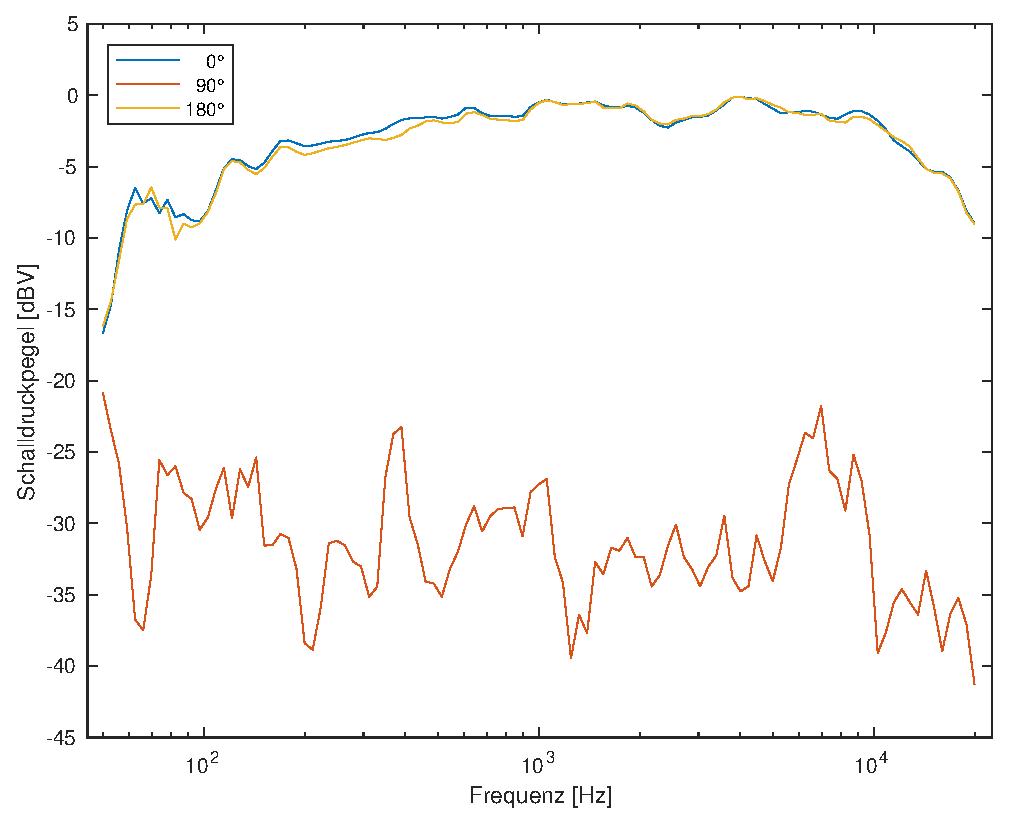
\includegraphics[width=0.95\linewidth]{Figures/km120_all}
    \end{subfigure}%
    \begin{subfigure}{.5\textwidth}
        \centering
        \caption{SM58}
        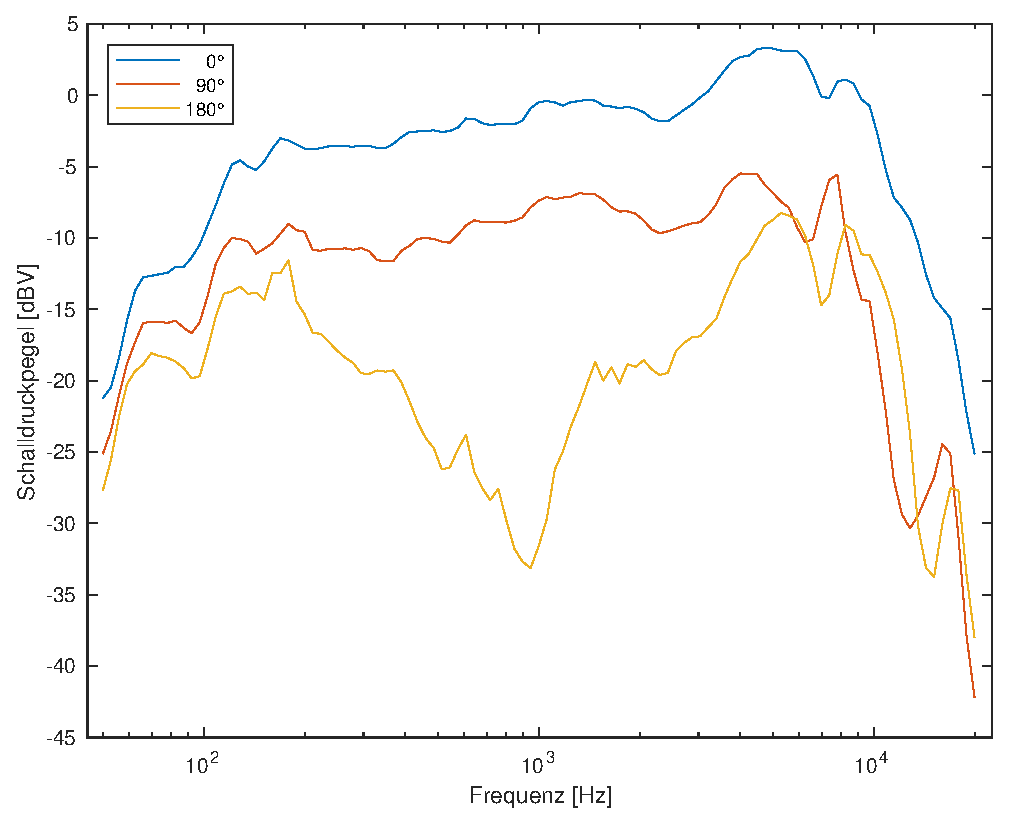
\includegraphics[width=0.95\linewidth]{Figures/sm58_all.eps}
    \end{subfigure}
    \caption{Geglättete Frequenzgänge aus drei verschiedenen Einfallsrichtungen}
    \label{fig:freq_all}
\end{figure}


\subsection{Richtcharakteristik}
Die frequenzabhängigen Richtcharakteristiken des Neumann KM184 sind in den Abbildungen ??? zu sehen.
Die Richtcharakteristik liegt je nach Frequenz zwischen breiter Niere und Niere. 
Die Richtcharakteristiken bei 125 Hz hat die Form einer breiten Niere, die Charakteristiken zwischen 250 Hz und 8000 Hz sind nierenförmig und bei 16000 Hz erkennen wir eine Superniere.
Beim Vergleich mit den frequenzabhängigen Charakteristiken auf www.neumann.com können wir keine deutlichen Unterschiede erkennen.
\subsection{Bündelungsgrad}
Der frequenzabhängige Bündelungsgrad des Neumann KM184 ist in Abbildung ??? dargestellt. 
Laut dem Handbuch der Audiotechnik (cite!!) hat eine Niere gemäß der Berechnung mithilfe der idealisierten Richtcharakteristik $A + B \mathrm{cos}(\theta)$ den Bündelungsgrad 3, eine breite Niere den Bündelungsgrad 1,89 und eine Superniere den Bündelungsgrad 3,73.
Demnach nähert sich der mit der Frequenz moderat steigende Bündelungsgrad des KM184 zwischen 100 Hz und ca. 5000 Hz zunehmend dem einer Niere an.
Dann kommt es zu einem Einbruch zwischen ca. 6000 Hz und 10000 Hz, wo der Bündelungsgrad bis auf einen für eine breite Niere typischen Wert abfällt. 
Für höhere Frequenzen steigt $\gamma$ nochmal stark an und erreicht  Super- und Hypernierentypische Werte.
